
\chapter{Evaluación subjetiva del códec}\label{capit:cap2}
\vspace{-2.0325ex}%
\noindent
\rule{\textwidth}{0.5pt}
\vspace{-5.5ex}% 
\newcommand{\pushline}{\Indp}% Indent puede ir o no :p

Las pruebas matemáticas presentadas al final del capítulo anterior no son las más relevantes para evaluar completamente la calidad de un codificador de audio. Es importante que el público auditor logre valorar su percepción con respecto al funcionamiento del producto realizado. En efecto, la señal ha sufrido diversos procedimientos de compresión con pérdidas y se vuelve necesario describir en qué medida éstas la han afectado.

Un test subjetivo que ha trascendido entre expertos de audio y diseñadores de códecs es el descrito por la recomendación BS.1534-11 del ITU-R \cite[]{series2014}, conocido también como MUSHRA (acrónimo del Inglés \emph{Multiple stimuli with hidden reference anchor}). 

MUSHRA es una prueba que, como su nombre lo indica, emplea múltiples \emph{estímulos}, los cuales son diferentes señales que han sido previamente codificadas y por lo tanto han sido distorsionadas por el codificador de audio diseñado. Se le presenta al oyente una referencia (señal original) y una versión oculta de ésta (es decir, no se le indica como tal), la cual se muestra en forma aleatoria en conjunto con el resto de las señales distorsionadas (anclas).

Las anclas son otras versiones codificadas de la señal con niveles perceptibles de degradación, las cuales tienen como propósito ajustar la escala de valores del oyente lo más posible a la escala absoluta, asegurándose que éste ha marcado con una puntuación más baja las muestras claramente más pobres y con una puntuación alta a las muestras claramente mejores. Dicha distorsión es realizada de manera intencional.

En esta sección se describirán los pasos para realizar el test MUSHRA como valoración subjetiva a las señales de audio codificadas, se valorarán los resultados obtenidos enunciando diversas conclusiones sobre los mismos.

\section{Selección de las señales de prueba}
Para la realización de las pruebas subjetivas del códec, MUSHRA recomienda seleccionar estímulos y/o señales de audio bajo los siguientes requerimientos:
\begin{itemize}
	\item Duración no mayor a 20 segundos.
	\item No seleccionar un número mayor a 10 estímulos para comodidad del oyente.
	\item Una versión de la referencia pasada por un filtro paso bajas a 3.5 kHz, situada en alguna de las anclas.
\end{itemize}
La primera recomendación se cumple, ya que las señales de la base no rebasan los 5 segundos. En el caso del segundo requerimiento se ha decidido seleccionar a los siguientes 5 estímulos debido a considerarse los mejores en calidad desde la codificación:
\begin{itemize}
	\item Apertura normal del S2.
	\item S4.
	\item Apertura normal del S1.
	\item S3.
	\item Murmullo pansistólico.
\end{itemize}

Las anclas son versiones de las señales anteriores codificadas bajo los formatos MP3 \cite[]{Noll1997} y OPUS \cite[]{Valin2010a}, otra versión con 30 dB de AWGN (ruido blanco gaussiano aditivo), la versión cifrada utilizando el códec propuesto y en efecto la referencia oculta (versión WAV). Las condiciones para estos formatos fueron tasas de datos de 8 kilobits por segundo CBR (excepto WAV), 16 bits por muestra y frecuencia de muestreo de 8,000 Hz. Las anclas con versión pasabajas no son realizables en el caso del audio cardiaco, ya que ninguna de estas señales rebasa en ancho de banda los 3 kHz y dicha diferencia no resultará audible.

\section{Procedimiento de evaluación MUSHRA}
\subsection{Preparación de la interfaz gráfica }
Se realizó por medio del software MAX\copyright~una interfaz gráfica adaptada al test MUSHRA \cite[]{Hummersone2011}. Por medio de esta interfaz el usuario califica la calidad de la señal de audio mostrada en alguno de los 5 canales con respecto a la referencia (canal R) con notas en una escala de 0 a 100 y relacionando los adjetivos calificativos: 0 a 20 si la calidad es \emph{mala}, 20 a 40 si la calidad es \emph{mediocre}, 40 a 60 si la calidad es \emph{regular}, 60 a 80 si la calidad es \emph{buena} y 80 a 100 si es de una \emph{excelente} calidad. 

Se define un estímulo por página, donde se podrán reproducir las anclas y la referencia cuantas veces sea necesario para el oyente. Cada una de las anclas está situada de manera aleatoria con el propósito de establecer el criterio de la \emph{referencia oculta}. La interfaz gráfica está diseñada para que no sea posible calificar algún ancla mientras no se esté reproduciendo. Se permitirá cambiar de página y/o estímulo una vez que todas las anclas en ésta hayan sido calificadas.

La Figura \ref{mushra} muestra la visualización en pantalla de la interfaz MUSHRA adaptada desde MAX\copyright~para la evaluación subjetiva del códec diseñado.
 % ------------------------------------------------
\begin{figure}[h!]
  \centering
  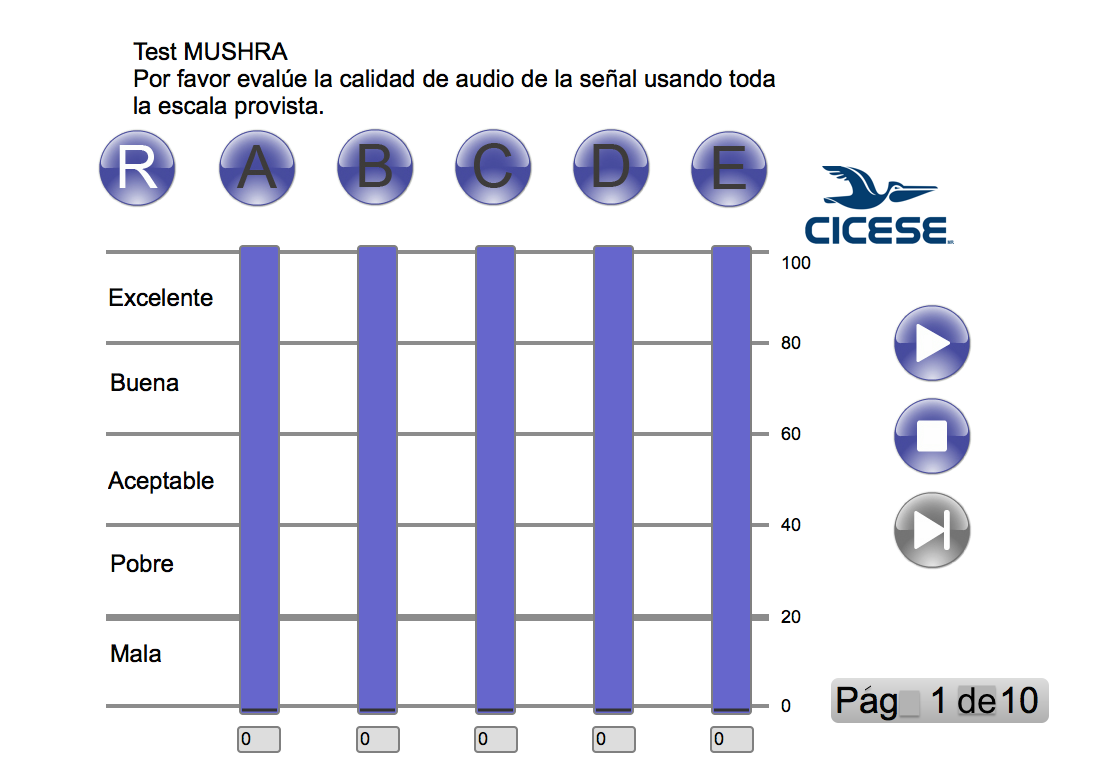
\includegraphics[scale=0.45]{mushra_interfaz.png}
  \caption{Visualización en la pantalla de la interfaz MUSHRA.}
  \label{mushra}
\end{figure}
% ---------------------------------------------

Las calificaciones otorgadas por cada uno de los oyentes son guardadas al terminar la prueba.

\subsection{Fase de adiestramiento}

Es importante la familiarización de los oyentes con las señales de audio empleadas en la prueba, el entorno (manejo de la interfaz), las herramientas empleadas y el procedimiento a realizar. Con esto los sujetos serán capaces de haber adquirido el conocimiento y las capacidades necesarias para apreciar y valorar con objetividad cada uno de los estímulos aportando información relevante a la prueba. 

La condición auditiva de los oyentes se ve fortalecida mediante una fase previa de adiestramiento, la cual se definió para este caso en la pre-evaluación de 3 de los estímulos sin considerar estas calificaciones para la valoración formal final. 

\subsection{Condiciones de audición}
Se han empleado para la prueba auriculares de estudio de calidad profesional con las siguientes características:
\begin{itemize}
	\item Marca: audio technica.
	\item Modelo: ATH-M50X.
	\item Respuesta en frecuencia: 15-28,000 Hz.
	\item Sensibilidad: 99 dB.
	\item Máxima potencia de entrada: 1,600 mW a 1 kHz.
	\item Impedancia de 38 ohms
\end{itemize}

Las pruebas fueron realizadas en un ambiente libre de ruido, con un clima agradable y fresco. Se percató que los oyentes no estuviesen bajo circunstancias no favorables en cuanto a salud o estado anímico. 

\subsection{Selección de los oyentes}
Según la experiencia, los datos procedentes de alrededor de 20 sujetos son suficientes para extraer conclusiones adecuadas de la prueba. Sin embargo, aumentando el tamaño de oyentes, y en partícular si son experimentados, es más conveniente. 
La inserción de una técnica de rechazo ya sea anterior (preselección) o posterior (postselección) a la prueba real resulta conveniente en ocasiones, ya que los resultados pueden sesgarse.  

Se han seleccionado 20 sujetos para la realización de las pruebas mostradas en este trabajo de tesis, los cuales son estudiantes de posgrado del CICESE. Estas personas participaron de manera voluntaria y no recibieron compensación económica alguna por su participación.

Las edades de los oyentes se encuentran en el intervalo de 22 a 34 años, presentando una edad promedio de 24.95 años y una desviación estándar de 2.84 años entre ellos. Cabe destacar que el 20\% de los participantes son del sexo femenino y el 10\% de ellos cuenta con alguna formación musical. Ninguno de los participantes presentó problemas de audición ni locomoción durante la prueba, cuya duración promedio fue de 15 segundos.

\section{Análisis estadístico de los resultados obtenidos en la prueba}
La calidad del funcionamiento medio de cada uno de los estímulos propuestos en esta investigación es identificada por medio del análisis estadístico de los resultados obtenidos, de igual manera puede corroborarse por medio de ello la fiabilidad de cualquier diferencia entre los valores que han sido obtenidos. 

El primer paso en el análisis estadístico consiste en clasificar los datos en una matriz ordenada como la siguiente:
\begin{equation}
\left[
\begin{array}{l c c c r}
		          & Sujeto_{1}	& Sujeto_{2} & \cdots & Sujeto_{n} \\
Audio_{1} 		& x_{1,1} 	& x_{1,2}      & \cdots & x_{1,n} \\
Audio_{2} 		& \vdots 	& \vdots & \vdots & x_{2,n} \\
\vdots 		& \vdots 	& \vdots & \cdots & \vdots \\
Audio_{m} 		& x_{m,1}	& x_{m,2} & \cdots & x_{m,n} \\
\end{array} \right] 
\end{equation}

De esta manera es más sencillo identificar las dispersiones individuales por sujeto, así como las calificaciones promedio de cada señal de audio evaluada. 
\subsection{Cálculo de los histogramas e intervalos de confianza}
La concentración de los valores medios de cada señal de audio presentan cierto grado de incertidumbre, asociado a los grandes rangos de valoración existentes para la prueba. Este grado de incertidumbre puede ser calculado y medido por medio de los \emph{intervalos de confianza}, los cuales expresan un rango de valores con los que se puede comparar la incertidumbre entre las valoraciones medias de los diversos estímulos empleados. 

Para el cálculo de los intervalos de confianza, se requiere la siguiente información:
\begin{itemize}
	\item Niveles de confianza
	\item Estadística
	\item Margen de error
\end{itemize}
Dadas estas tres entradas, el conjunto de valores del intervalo de confianza se define por la $muestra \pm margen~de~error$, y la incertidumbre asociada con el intervalo de confianza se especifica por el nivel de confianza.

El cálculo de los intervalos de confianza puede definirse en los siguientes cuatro pasos:
\begin{itemize}
	\item Identificar/seleccionar una muestra estadística que se desea emplear para estimar como parámetro (media, desviación estándar).
	\item Seleccionar un nivel de confianza. Es necesario describir el grado de incertidumbre de algún método de muestreo. Frecuentemente en las investigaciones se elige el 90\%, 95 \% ó 99\% de niveles pero cualquier porcentaje puede ser utilizado.
	\item Encontrar el margen de error, el cual es el producto del valor crítico y la desviación estándar en la estadística. Para una distribución normal con $n$ elementos el error estándar puede definirse como:
		\begin{equation}
		STD_{e}  = \frac{\sigma}{n},
	\end{equation}
donde $$\sigma=\sqrt{\frac{1}{N}(x_{i}-\mu)^2}$$ 
es la desviación estándar del conjunto de $n$ elementos $x_{i}$ con media $\mu$.
	\item Especificar el intervalo de confianza. La incertidumbre es denotada por el nivel de confianza, y el rango del intervalo de confianza se define por medio de la siguiente expresión:
	\begin{equation}
		IC = muestra  \pm margen~de~error,
	\end{equation}
	lo cual demuestra que una población de mayor número $n$ de elementos estadísticos evaluados denotará un menor margen de error y proporcionalmente mejores intervalos de confianza calculados.
\end{itemize}

Para los estímulos seleccionados en esta prueba se han calculado las calificaciones medias de los 20 oyentes (sujetos) y se han calculado los histogramas e intervalos de confianza correspondientes a un nivel de confianza del 95\%. Las Figuras \ref{IC_NS1}, \ref{IC_NS2}, \ref{IC_S3}, \ref{IC_S4}, y \ref{IC_PM} muestran los resultados obtenidos.

 % ------------------------------------------------
\begin{figure}[h!]
  \centering
  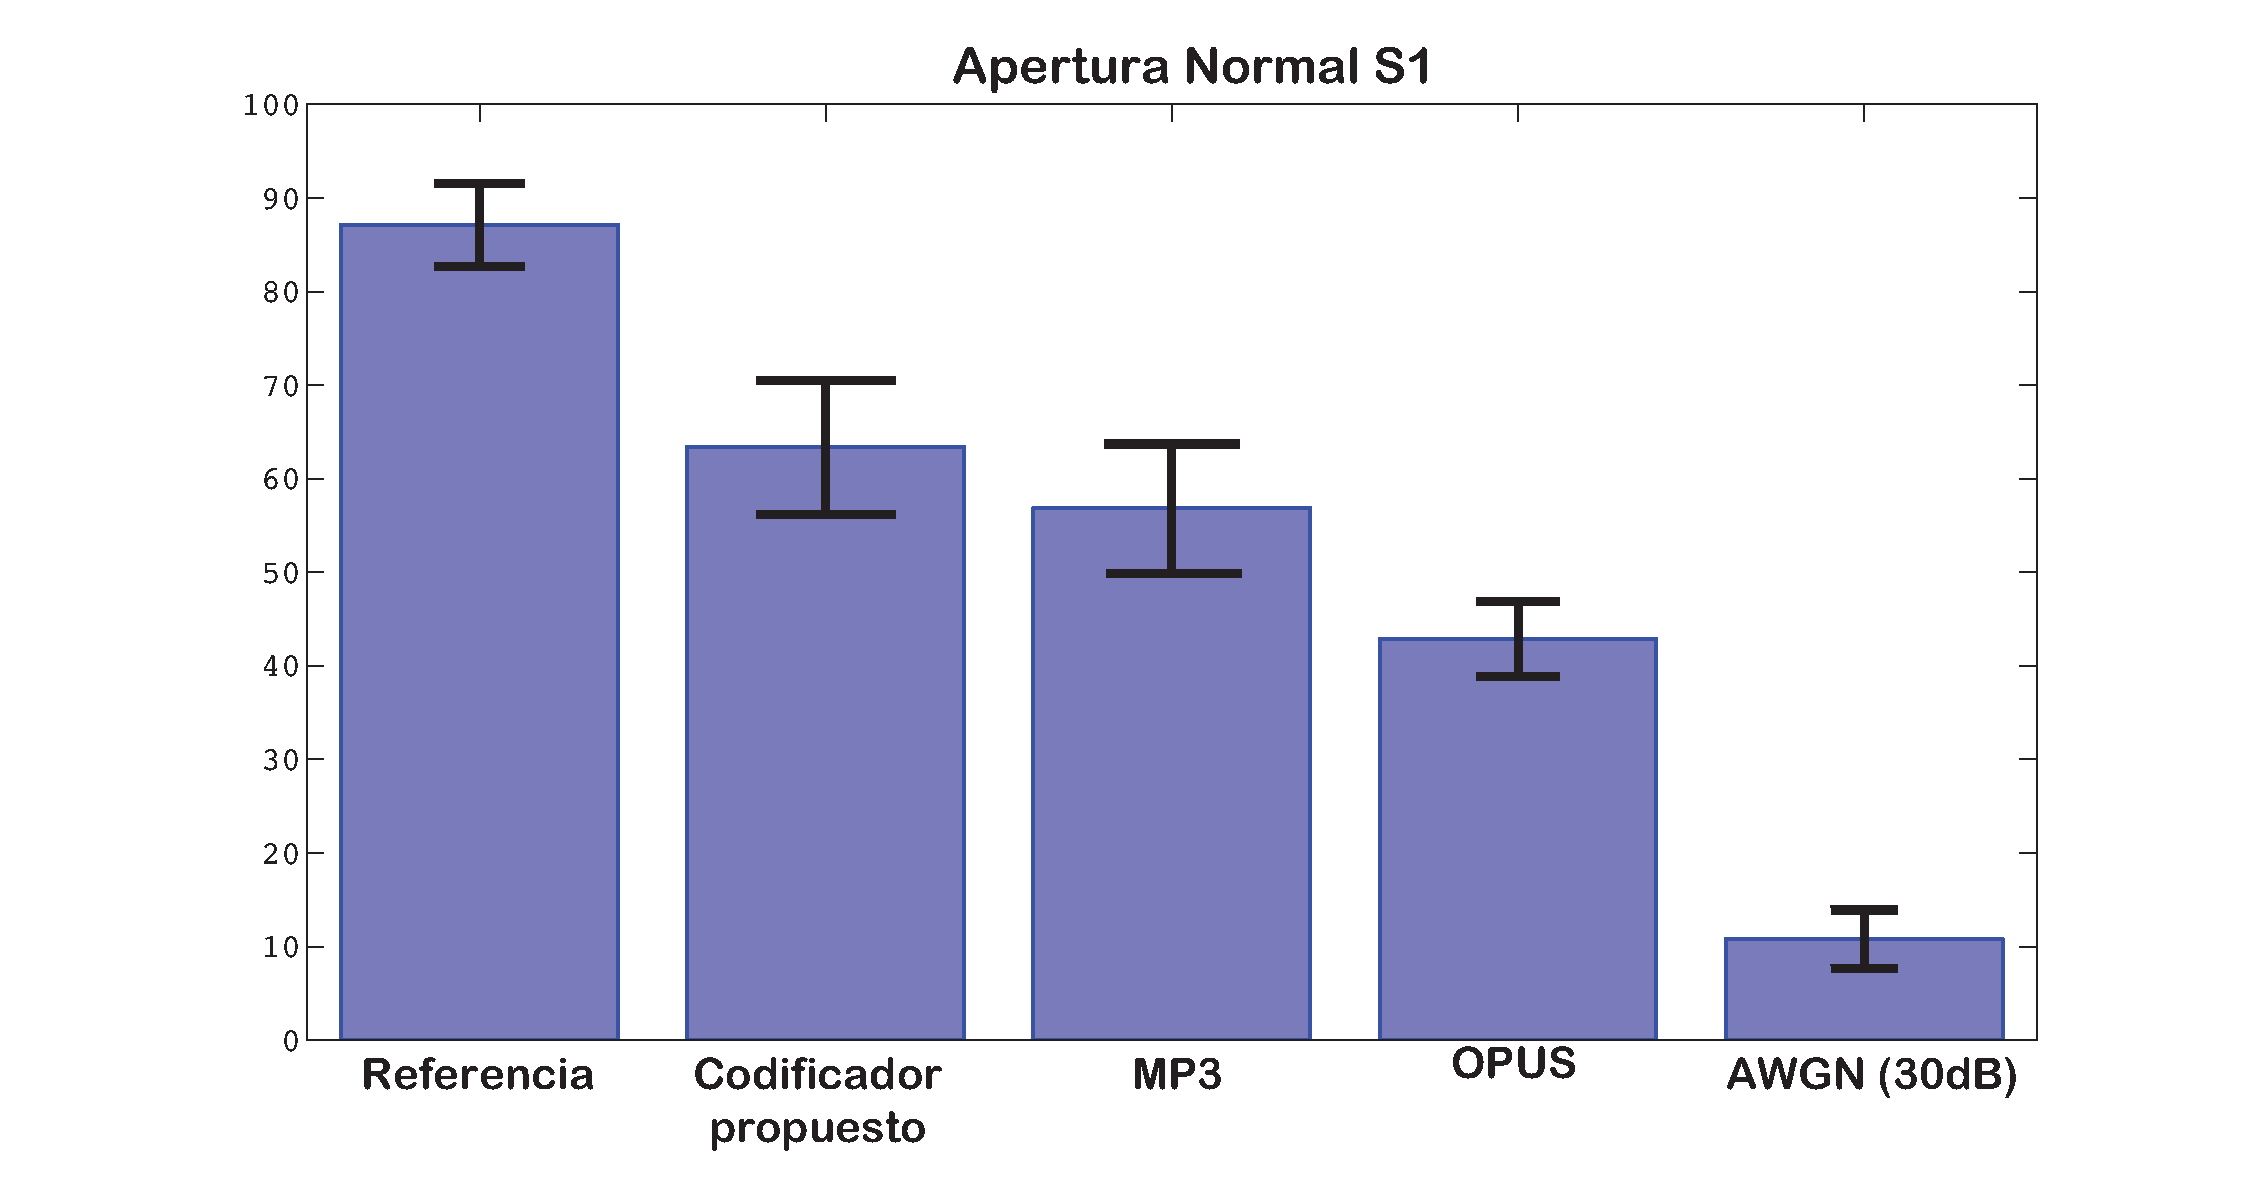
\includegraphics[scale=0.38]{IC_NormalSplitS1.eps}
  \caption{Histograma de las calificaciones medias e intervalos de confianza para el estímulo Apertura Normal S1.}
  \label{IC_NS1}
\end{figure}
% ---------------------------------------------
 % ------------------------------------------------
\begin{figure}[h!]
  \centering
  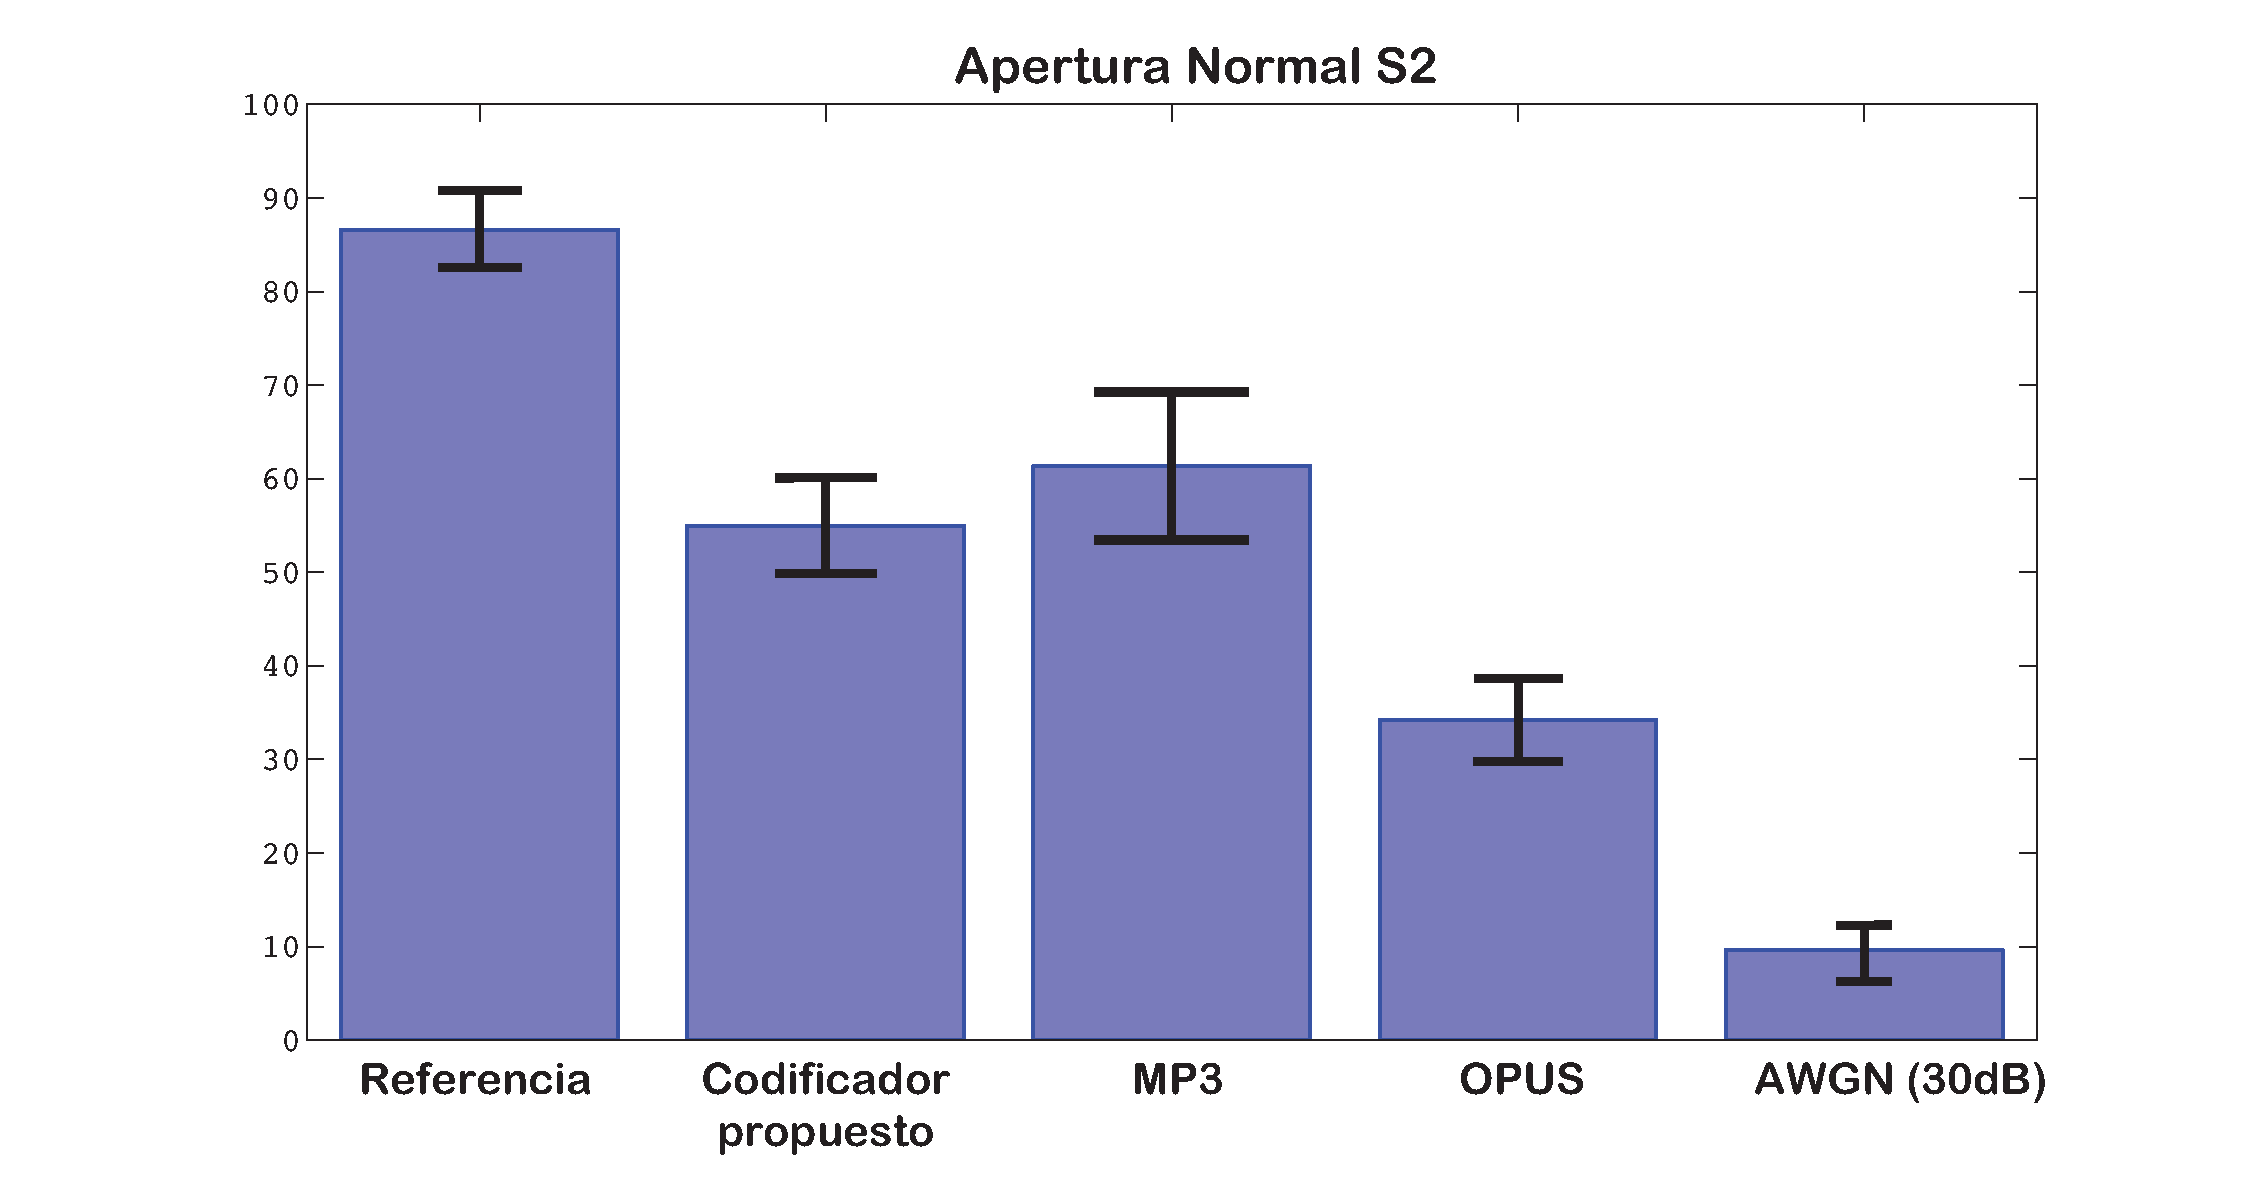
\includegraphics[scale=0.38]{IC_NormalSplitS2.eps}
  \caption{Histograma de las calificaciones medias e intervalos de confianza para el estímulo Apertura Normal S2.}
  \label{IC_NS2}
\end{figure}
% ---------------------------------------------
 % ------------------------------------------------
\begin{figure}[h!]
  \centering
  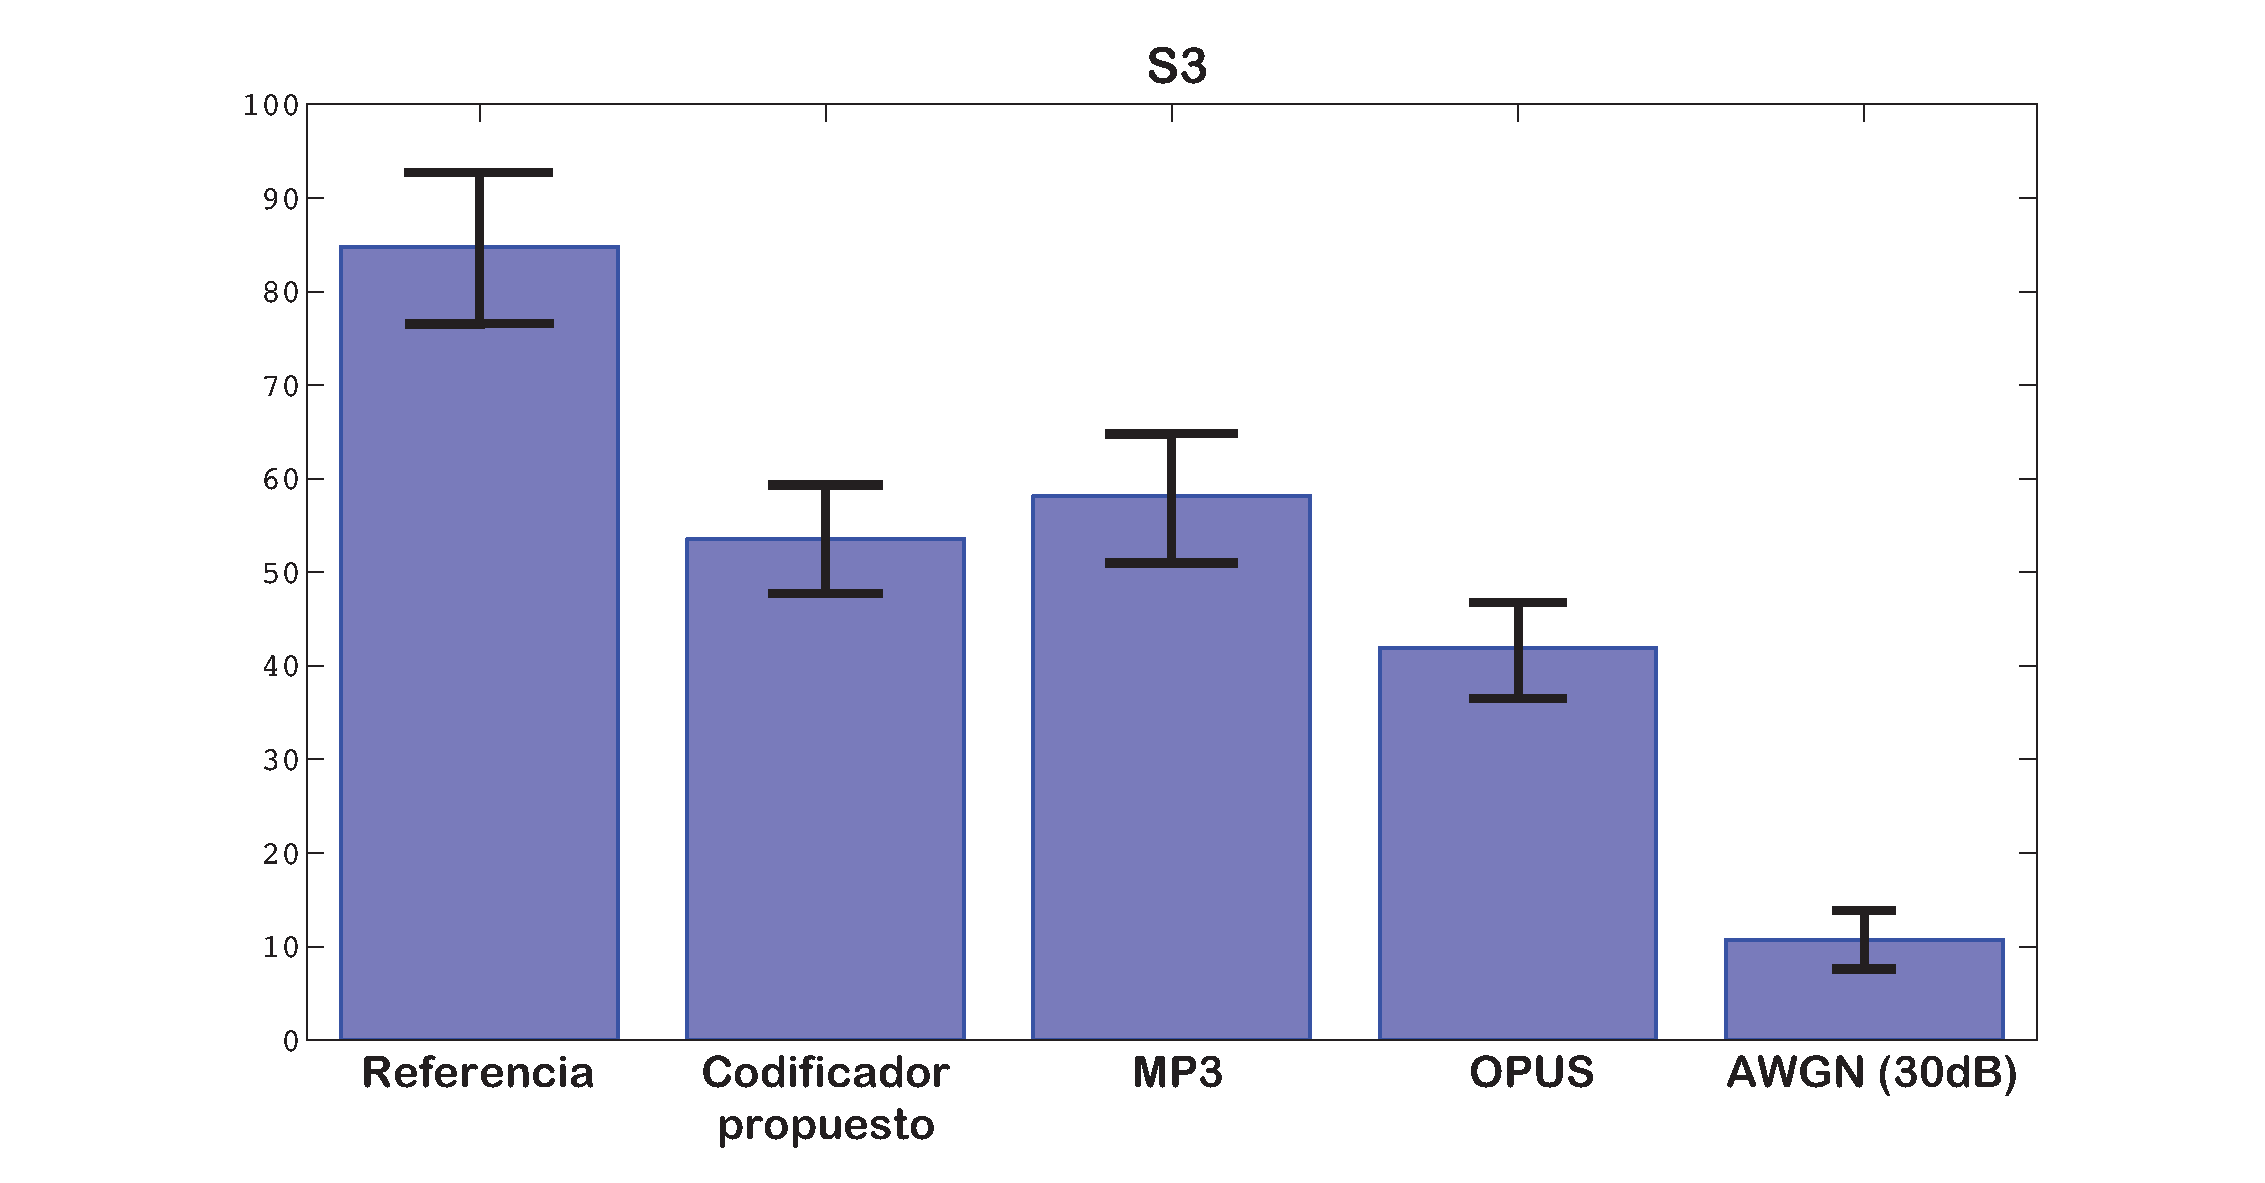
\includegraphics[scale=0.38]{IC_S3.eps}
  \caption{Histograma de las calificaciones medias e intervalos de confianza para el estímulo S3.}
  \label{IC_S3}
\end{figure}
% ---------------------------------------------

 % ------------------------------------------------
\begin{figure}[h!]
  \centering
  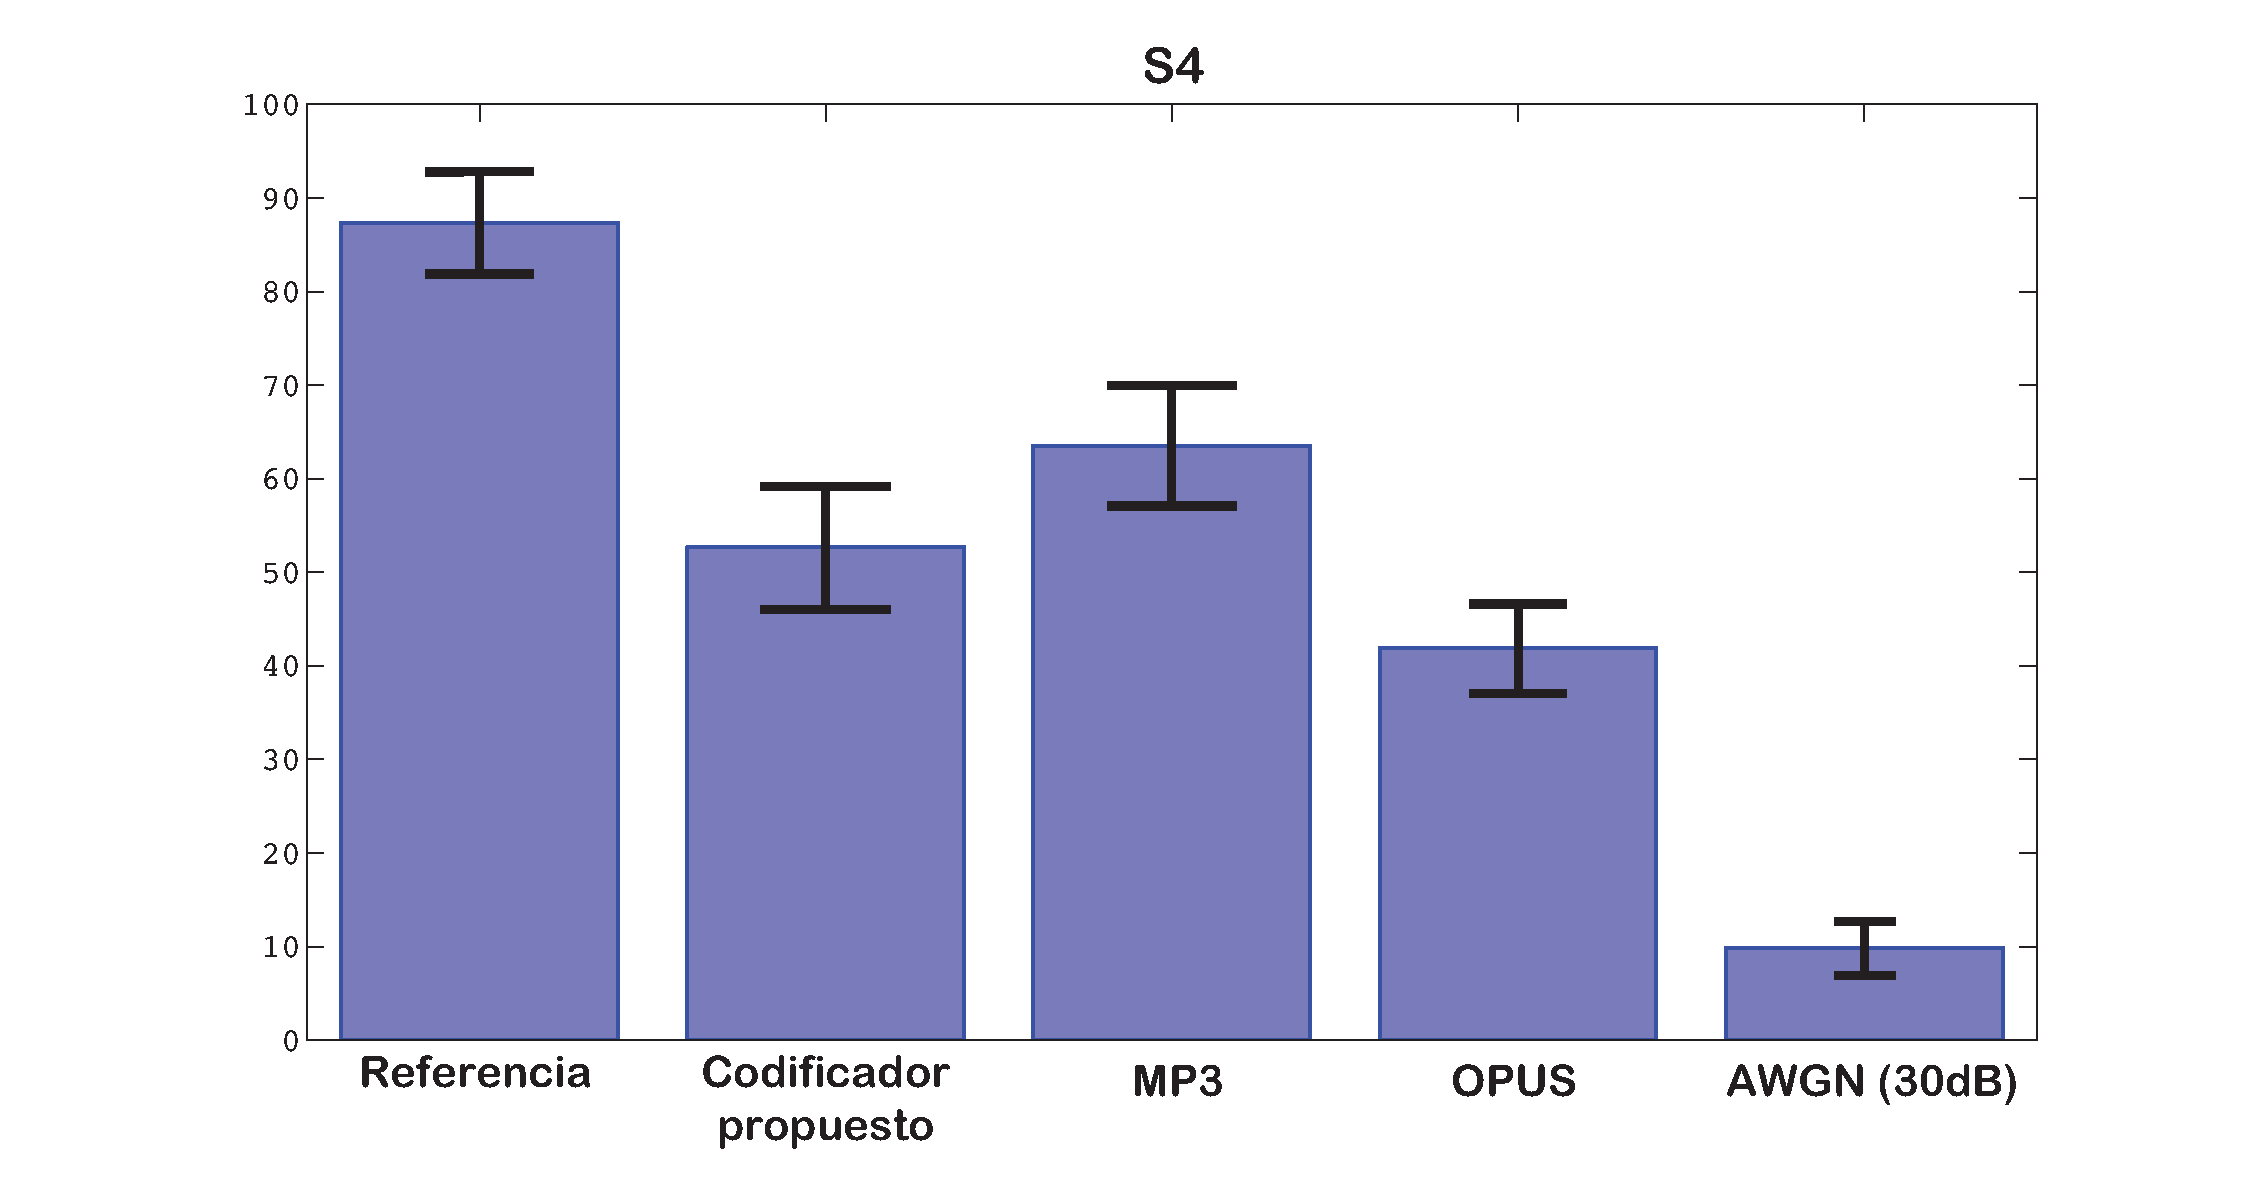
\includegraphics[scale=0.38]{IC_S4.eps}
  \caption{Histograma de las calificaciones medias e intervalos de confianza para el estímulo S4.}
  \label{IC_S4}
\end{figure}
% ---------------------------------------------
 % ------------------------------------------------
\begin{figure}[h!]
  \centering
  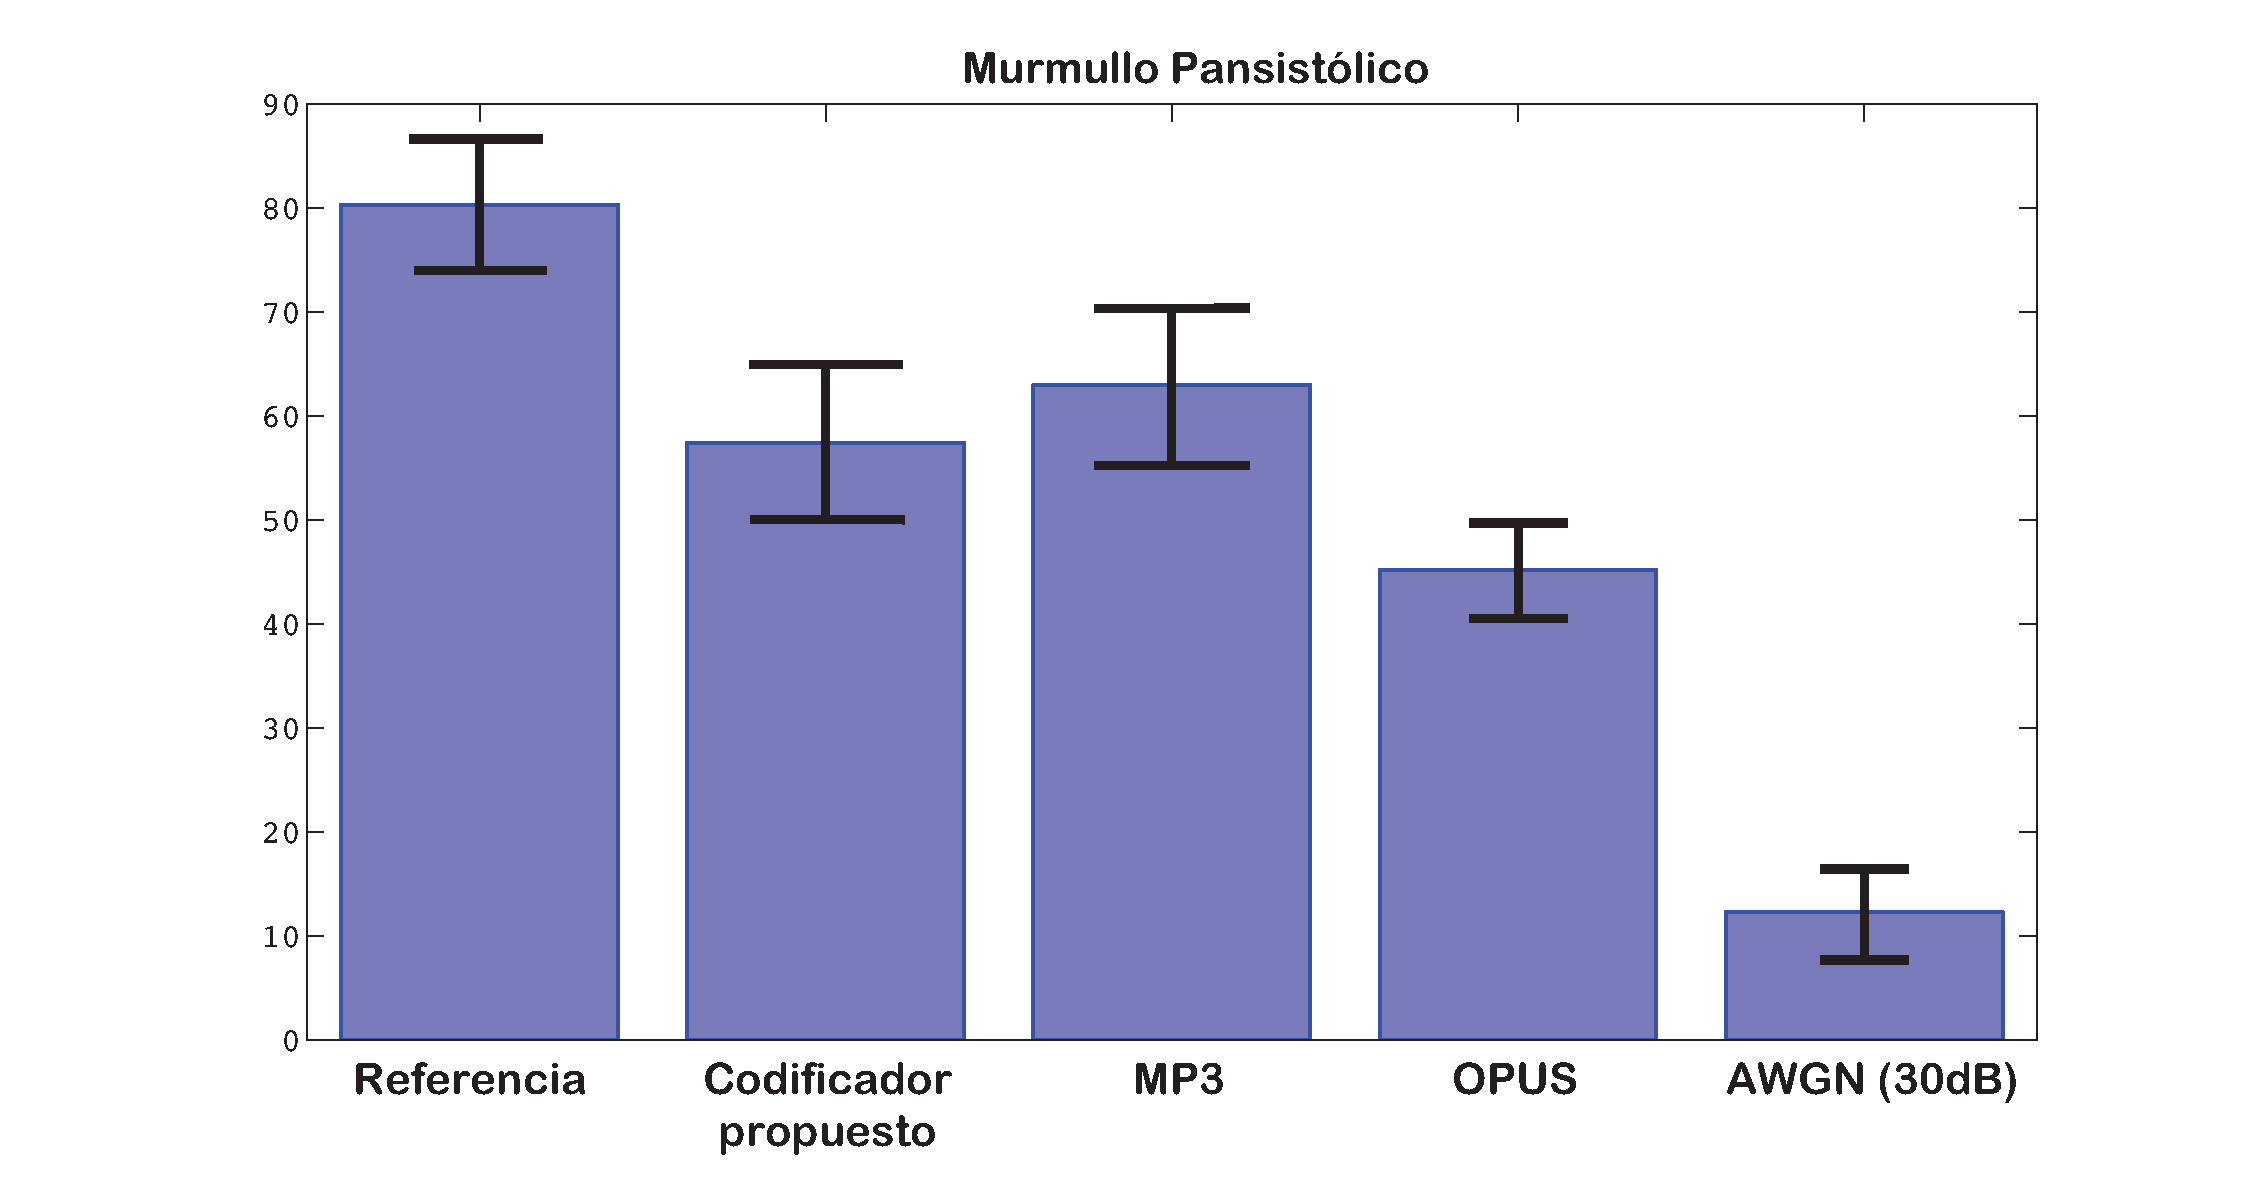
\includegraphics[scale=0.38]{IC_PansistolycMurmur.eps}
  \caption{Histograma de las calificaciones medias e intervalos de confianza para el estímulo Murmullo Pansistólico.}
  \label{IC_PM}
\end{figure}
% ---------------------------------------------

 Los resultados arrojados por la prueba avalan el buen desempeño del codificador diseñado en este trabajo de tesis, cuya valoración promedio se encuentra en el intervalo de \emph{aceptable} (40 a 60) según la escala MUSHRA. Como se indicó en un principio, la referencia o señal original obtuvo la calificación más alta posible para todos los estímulos. Por otro lado, la versión con ruído aditivo fue calificado con la nota más baja. La prueba fue intencionada para que estos resultados se ocurrieran y existiesen calificativos más cercanos para las otras anclas. 

 En las Figuras puede observarse que, aunque las versiones de MP3 en la mayoría de los estímulos superan en calificación promedio al códec (excepto en la Apertura normal del S1), de manera estadística los intervalos de confianza son muy cercanos entre estas dos anclas. En contraste, la versión codificada por OPUS presentó calificaciones más bajas, y en este caso los intervalos de confianza no lograron acercarse en ningún estímulo a los del codificador.
 
 Es importante mencionar que los codificadores MP3 y OPUS utilizan técnicas de codificación entrópica (no empleando ninguna en el codificador diseñado) y técnicas de cuantificación más sofisticadas que las empleadas en esta propuesta. A pesar de no haber implementado estos métodos en el códec, su calidad subjetiva fue evaluada como aceptable y competente\footnote{Los intervalos de confianza entre el codificador y MP3 fueron muy cercanos.} en todos los estímulos evaluados en la prueba. 
 
 Los resultados arrojados por la prueba MUSHRA para el codificador propuesto deben tomarse con cautela,son los especialistas en la salud quienes en realidad valorarán si la calidad perceptual otorgada por el codificador diseñado es la necesaria para que pueda realizarse la compresión, representación y transmisión de fonocardiogramas por el mismo. 
 
 De igual manera, los oyentes expertos en salud podrán determinar si las anomalías cardiacas son aún diagnosticables al realizar estos procedimientos. De igual manera los analistas clínicos podrán catalogar si los artefactos introducidos por el códec pueden detectarse como cardiopatías. Ninguno de los participantes seleccionados para el desarrollo de esta prueba tiene conocimientos especializados de este tipo. 
 
 A partir de estos resultados se formularán conclusiones importantes en la siguiente sección, ya que esta investigación ha desarrollado un codificador adaptado a una señal biológica importante para el diagnóstico clínico. 
 
 



